% !TeX root = ../main.tex
% Add the above to each chapter to make compiling the PDF easier in some editors.

\chapter{Introduction}\label{chapter:introduction}

% TODO: short text. motivation + RQ.
% cloud erwähnen.
% statisch vs dynamic eam
% forziert dazu ead zu evolutionieren

\section{Motivation}
%although satz nochmal überarbeiten
Companies operate in a dynamic marketplace defined by fast-changing technologies, shortened product life cycles and increasing specialization and competition in global value chains. The ability to adapt to the changing environment has become fundamental for companies to have an advantage over the competitors. 
However, when organizations try to adapt to create an advantage it results in a more complex landscape within the enterprise. The landscape becomes more heterogeneous when trying to incorporate new methodologies, technologies and tools. This leads to an incompatible landscape of incompatible and costly information systems, business processes and organizational structures. \hl{(Strategic Enterprise Architecture Management: Challenges, Best Practices ...)}

Over the last decade EAM has become a strategic advantage regarding the rapidly developing markets. One of the functions of EAM is to create transparency of the application landscape within the enterprise, reduce the landscape complexity and its costs.

% in manually add: collected in a file and imported to EA tool?
In order to achieve these goals, a highly accurate, consistent and uniform EA documentation is needed. However, EA often ends up with a scarce documentation.\hl{(Hauder Current Practices 2013)} EA documentation is one of the main problems when it comes to the collection of EA information, since most of the information is collected manually. Today's EA documentation is a very complex process due to the immense application landscape consisting of redundant and inconsistent data. The collection process is contemplated as very time consuming  process and the data quality is insufficient. %insufficient?
Most of the organizations have no dedicated process for the collection of EA information which confirms the that the lack of governance in EA projects is one of the major challenges since it is difficult to document information for a "plethora of stakeholders". \hl{(Hauder Empirical Analysis) (Lucke, Critical Issues in Enterprise Architecting...) } Some organizations have tried to automate the process of EA documentation but the automated process is mostly limited to import manually a file which contains manually collected data/information. 
Organizations should aim for a direct integration of information sources into EA Tools and target an automated EA documentation of external information sources such as cloud providers. 
According to a cloud computing survey in 2016 companies are investing in cloud solutions to lower costs and replace legacy system. The benefits of cloud computing are that organizations do not need to buy infrastructure anymore which signifies considerable reduction on installation and maintenance of computing infrastructure costs.\hl{(IDG Executive Summary. Cloud Computing Survey. 2016)}

Some organizations show the attempts of an automated EA documentation using Network Scanners and ESBs but the information concludes to be incomplete and not up-to-date. 
The use of external information sources such as cloud providers will increase the actuality and data quality of the information delivering structured static and dynamic data enriching the EA Tool. In order to obtain that changes in cloud-based environments (as ext. information sources) should update the EA documentation.
% As proposed in survey by \hl{Hauder et al} the EA
% mapping between information sources and meta model
% focus on automated documentation
% focus external sources such as cloud. cloud becoming important for focus on core competences
% enrich ea tool con static y dynamic data
% Control room concept of Brückmann as monitoring?
% \hl{ ... }
% doerst aussage
In 2004, ter Doerst stated: "in 7 years from now, enterprise architecture will be a real-time tool for management and redesign of the enterprise for better performance, flexibility and agility". (ter Doerst, Tool Support for Enterprise Architecture)
As shown in the survey of \hl{Hauder et al.} organizations are far away from using an EA Tool as a real-time tool. This thesis will propose a solution for improving the EA documentation regarding external sources, specially applications running in a cloud-based environment. Since lack of governance is one of the leading problems in EA this thesis will propose some guidelines % name conventions
and a tool integration in the development pipeline to automate the documentation of cloud applications, enriching it by business specific information (Business domain assignments, \hl{...}) and enhance the documentation with dynamic data to enable a continuous process of monitoring application performance and infrastructure.
% integrating dynamic data: real-tool
% is still not like that.
% link to performance
% darueberhinaus monitoring para prozess de abajo.
% cover automated documentation ea goernance, cloud as ext services.
% para alcanzar todo eso integracion de toolchain an development pipeline
\hl{ ... }

\section{Research Questions}\label{section:researchquestions}
%Citation test~\parencite{latex}.

%\subsection{Research Questions}

To support this, the following research questions (RQ) will be answered during this thesis.

\textbf{RQ1. How to assign the application landscape to business domains?}
The first research question will demonstrate a solution approach to assign the business domain model to the application landscape.

\textbf{RQ2. How to obtain EA relevant information from the runtime behaviour of cloud-based environments?}
The goal of this research question is to identify what the possibilities are to obtain runtime information of applications running in a cloud-based environments and what information is relevant for EAM.

\textbf{RQ3. How to automate the assignment process with an integrated toolchain?}
The second research question will describe a process integrating the most common tools used within a company to automate the business assignments and the enterprise architecture documentation process.

\textbf{RQ4. How does a prototype implementation of the automated documentation process of cloud applications look like?}
To demonstrate that the automated documentation of application running in cloud-based environments is possible regarding the toolchain described in the question above (RQ3) this research question will describe a prototype implementation of the automated documentation process of cloud applications. The prototype implementation based on an open source project is an application and service inventory containing the EA relevant information and metadata of these. One of the technology trends mentioned before is Cloud migration. This reduces infrastructure and maintenance costs, reduces transparency but increases complexity of EA documentation due to the higher number of applications. The growing number of applications is therefore a challenge. To increase the independence of the teams and increase the reusability of these %applications
the open source project was expanded to answer questions like: Which service runs where? Which domain does it belong to? What does it do? Who is responsible for that?


\section{Approach}
This thesis is composed by a literature review and a case study of the solution proposal. The literature review is divided into 4 parts, the same as the case study phase. Figure 1.1 gives a clear overview of the research approach.

First the scope of research of this work will be described resulting in a set of research questions . The second part of the literature review is the topic conceptualization. The aim is to get an overview of EA and how data is collected in organizations and what technology trends affect the current documentation process. 
For the literature review part (scope of research, topic conceptualization, literature search and literature analysis)  an investigation according to the guidelines and the process model of Webster and Watson (2002) was carried out (Webster / Watson2002). The research relates to different terms or areas found in the second part: topic conceptualization. First, different terms have been identified to cover different aspects of each chapter. Among other things, a search with a number of combinations of the relevant terms was completed for the individual chapters.
The databases used for the search provide a variety of publications, which is why a broad coverage of the terms is possible. The databases used for this work are as follows:

\begin{itemize}
    \item ACM Digital Library
    \item Google Scholar
    \item IEEE Xplore / Electronic Library Online (IEL)
    \item University Library of the Technical University of Munich
\end{itemize}

For the search results the following search criteria were used in meaningful combinations:

\begin{itemize}
    \item Enterprise Architecture
    \item Enterprise Architecture Management
    \item Automated EA documentation
    \item Cloud Computing
    \item Continuous Delivery/ Integration
    \item Microservices
    \item Application Performance Monitoring
\end{itemize}

In addition, a backward search and a forward search were performed. This results in a larger total of results. Since the Technical University of Munich provides its students with a number of licenses, it is possible to use scientific research databases. The quality of the search results is ensured by the licenses for the databases and proves to be very helpful.

As marked before, organizations struggle with the documentation of their current state due to the o the immense application landscape consisting of redundant and inconsistent data. Organizations seek to automate that EA documentation process, that is why the focus of the literature will depict the approaches to automate the EA documentation process with the relevant data sources. These documentation processes are named and compared in the third and forth part of the literature review.

The second part of this work will suggest a new approach based on the approaches found in the literature. A new solution approach is introduced due to current research endeavours that lack in integrating cloud-based environments such as Platform as a Service (PaaS) and Software as a Service (SaaS) for automated EA documentation. 

The solution approach will include the technology trends that influence nowadays the EAM such as agile development (continuous delivery and integration), cloud aspects and decomposition of legacy systems into application components or microservices. Regarding the EAD, the advantages and the challenges are depicted. Once the solution approach has been develop it has to be analyzed and evaluated in a productive environment. For the development and evaluation phase of the solution approach an insurance company was examined regarding its process of EA documentation. The implementation phase of this work will target the Application Performance Monitoring (APM). Performance data is gathered during the EA documentation process and a set of metrics is generated based on the performance data. The performance of the application is measured using the metrics to conclude operation and strategic decisions for the EAM. It follows that improved EAM use cases can be derived from an automated EA documentation process taking into consideration APM. The proposed solution approach for automating Enterprise Architecture Documentation (EAD) by investigating major technology trends that influence EAM, how they affect EAM and how an automated EAD process can lead to improved EAM use cases.
\begin{figure}[htpb]
  \centering
  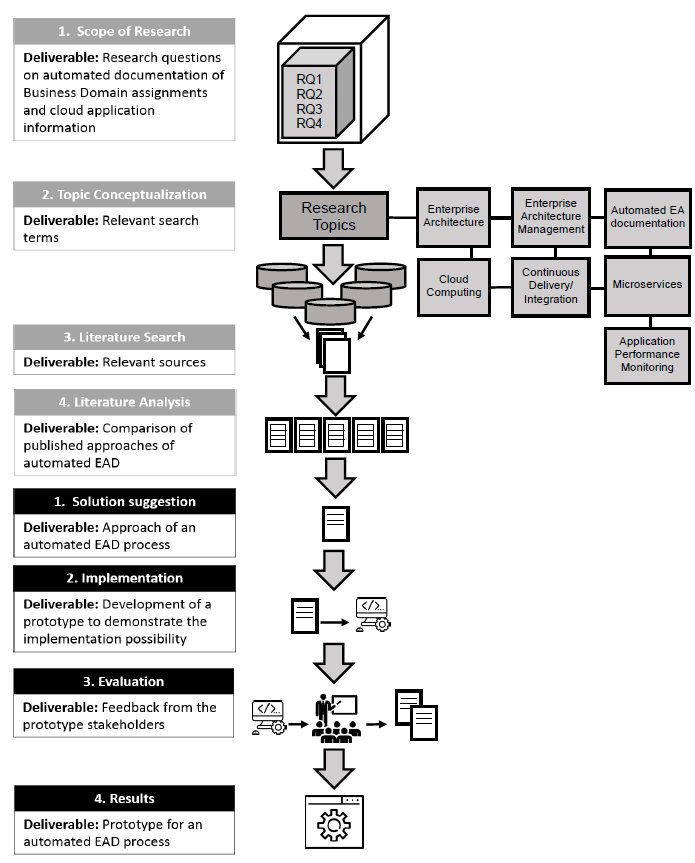
\includegraphics[width=0.8\textwidth]{figures/approach.PNG}
  \caption{Research approach~\parencite{Corpancho Villasana 2018}}
  \label{fig:research-approach}
\end{figure}